\documentclass[ucs]{beamer}
\usetheme{Frankfurt}
%\usefonttheme{serif}

\usepackage[T2A]{fontenc}
\usepackage[utf8]{inputenc}
\usepackage[english,russian]{babel}
\usepackage{amssymb, amsmath, amsfonts}
\usepackage{graphicx}
\usepackage{subfigure}
\usepackage{color}
\usepackage{multimedia}
\usepackage{tikz}
\usepackage{pgfmath}
\usetikzlibrary{arrows,fit,positioning,shapes.multipart}
\usepackage[percent]{overpic}


\usecolortheme[named=cyan]{structure}

\title{Компьютерные модели микронасоса Кнудсена на основе численного решения уравнения Больцмана}
\author{Мартынов Д.В.\inst{1}, Рогозин О.А.\inst{1}, Клосс Ю.Ю.\inst{2}, Черемисин~Ф.Г.\inst{3}}
\institute{
	\inst{1}Московский физико-технический институт (ГУ)\and
	\inst{2}Российский научный центр ``Курчатовский институт''\and
	\inst{3}Вычислительный центр РАН имени А.А. Дородницина
}
\date[NPNJ'2010]{8 международная конференция по неравновесным процессам в соплах и струях}

\newcommand{\Kn}{\mathrm{Kn}}
\newcommand{\dd}{\;\mathrm{d}}


\begin{document}

\begin{frame}
	\titlepage
\end{frame}

\begin{frame}
	\tableofcontents
\end{frame}

%%%%%%%%%%%%%%%%%%%%%%%%%%%%%%%%%%% Олег %%%%%%%%%%%%%%%%%%%%%%%%%%%%%%%%%%%%%

\section{Введение}

\subsection{Эффект теплового скольжения}
\begin{frame}
	\frametitle{Эффект теплового скольжения}
	англ. thermal transpiration (thermal creep)
	\begin{figure}
		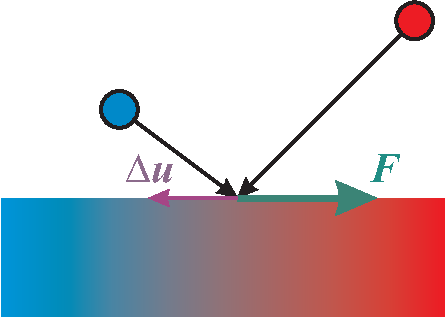
\includegraphics[height=3cm]{creep.pdf}
	\end{figure}
	\begin{block}{}
		\textbf{Reynolds O.} On Certain Dimensional Properties of Matter in the Gaseous State
		// Phil. Trans. Royal Soc. — 1879. — V.~170. — P.~727–845.
	\end{block}
	\begin{block}{}
		\textbf{Maxwell J.C.} On Stresses in Rarefied Gases arising from Inequalities of Temperature
		// Phil. Trans. Royal Soc. — 1879. — V.~170. — P.~231–256.
	\end{block}
\end{frame}

\begin{frame}
	\frametitle{Эффект теплового скольжения}
	\begin{itemize}
		\item тепловое скольжение вдоль стенок
		\item течение Пуазейля внутри канала
	\end{itemize}
	\begin{figure}
		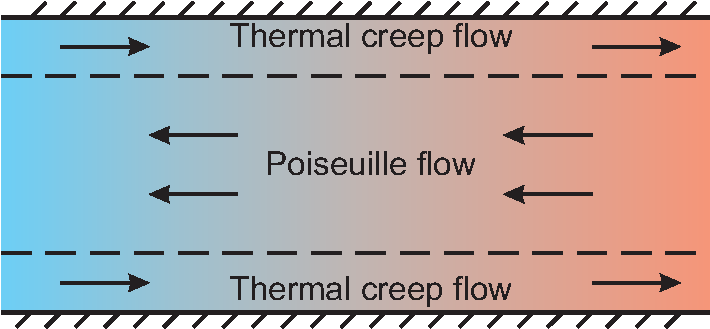
\includegraphics[height=4cm]{knudsen_flows.pdf}
	\end{figure}
\end{frame}

\subsection{Оригинальный насос Кнудсена}
\begin{frame}
	\frametitle{Оригинальный насос Кнудсена}
	\begin{block}{}
		\textbf{Knudsen M.} Eine Revision der Gleichgewichtsbedingung der Gase. Thermische Molekularströmung 
		// Ann. der Phys. — 1910. — Bd.~31, Nr.~9. — S.~205–229.
	\end{block}
	\begin{figure}
		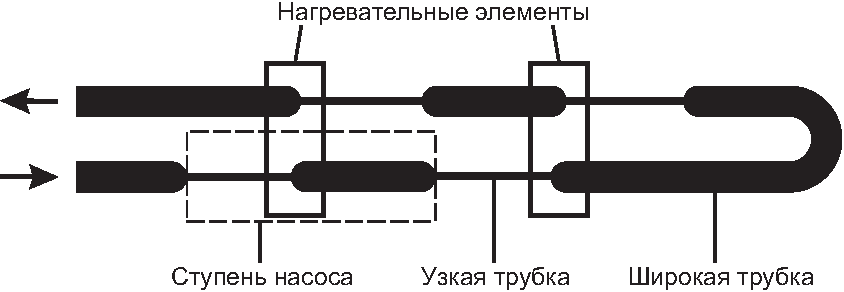
\includegraphics[width=10cm]{knudsen_device.pdf}
	\end{figure}
	\begin{itemize}
		\item соединяет 2 резервуара при \(T_1=T_2\), создавая \(P_1<P_2\)
		\item эффективно работает при числах Кнудсена \( \Kn=\dfrac{\lambda}{d} \sim 1\).
	\end{itemize}
\end{frame}

\subsection{Cовременные микронасосы Кнудсена}
\begin{frame}
	\frametitle{Различные модификации насоса Кнудсена}
	\begin{enumerate}[(a)]
		\item пластинчатый
		\item змейчатый
		\item аккомодационный
	\end{enumerate}
	\bigskip
	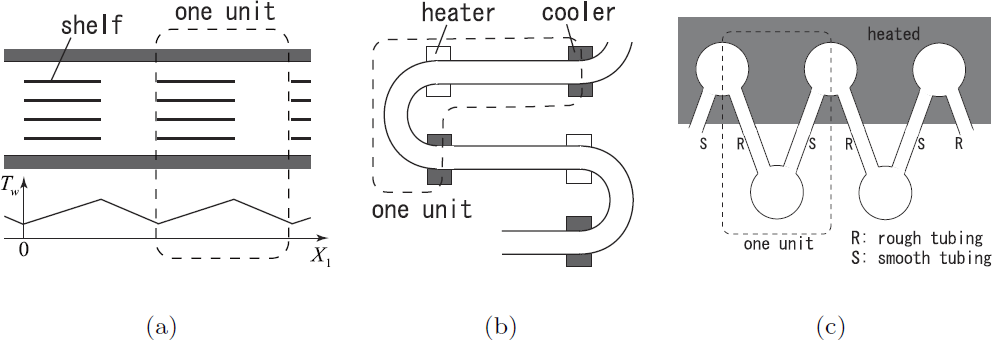
\includegraphics[width=\columnwidth]{pumps.png}
\end{frame}

\begin{frame}
	\frametitle{Лабораторный экземпляр}
	\begin{center}
		University of Southern California \\
		Department of Aerospace \& Mechanical Engineering
	\end{center}
	\begin{figure}
		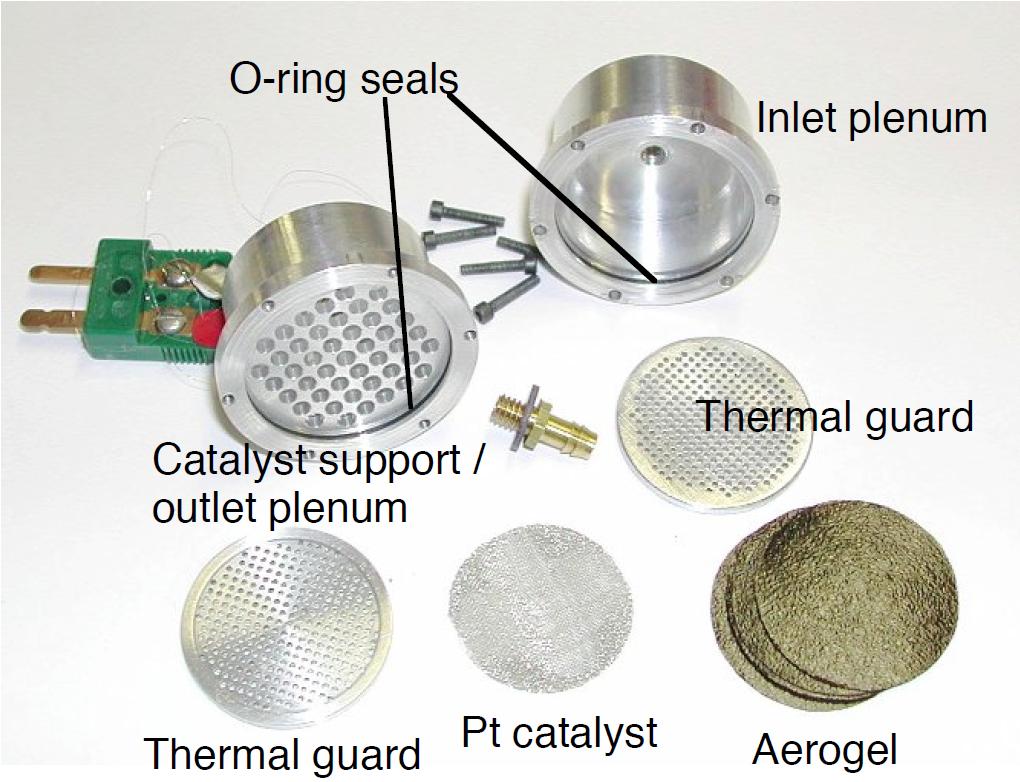
\includegraphics[width=8cm]{ModernInv.png}
	\end{figure}
\end{frame}

\section{Численные методы}

\subsection{Уравнение Больцмана}
\begin{frame}
	\frametitle{Численное решение уравнения Больцмана}
	Кинетическое уравнение Больцмана для одноатомного газа
	\[
		{\partial{f} \over \partial{t}} + \boldsymbol{\xi} \cdot {\partial{f} \over \partial\mathbf{r}} = 
		\int\limits_{\mathbb R^3} \int\limits_0^{2\pi} \int\limits_0^{b_m} 
		(f_1' f' - f_1 f) gb \dd{b} \dd\varepsilon \dd\boldsymbol\xi_1 \equiv J(f)
	\]
	\begin{itemize}
		\item статистические методы
		\begin{itemize}
			\item метод DSMC
		\end{itemize}
		\item конечно-разностные методы
		\begin{itemize}
			\item модельные уравнения (ES-BGK, Шахова, ...)
			\item \alert{прямой проекционный метод}
		\end{itemize}
	\end{itemize}
\end{frame}

\begin{frame}
	\frametitle{Расщепление уравнения Больцмана}
	\centering{Моделируем эволюцию функции распределения \(f(t,\mathbf{r},\boldsymbol\xi)\)}
	\newline\newline
	\begin{columns}[c]
		\begin{column}{5cm}
			\begin{enumerate}
				\item уравнение переноса
				\begin{itemize}
					\item \(\displaystyle{\partial{f} \over \partial{t}} + \boldsymbol\xi \cdot {\partial{f} \over \partial\mathbf{r}} = 0\)
				\end{itemize}
				\item интеграл столкновений
				\begin{itemize}
					\item \(\displaystyle{\partial{f} \over \partial{t}} = J(f)\)
				\end{itemize}
				\item вычисление макропараметров
				\begin{itemize}
					\item \(n = \int f \dd\boldsymbol\xi$
					\item \(\mathbf{u} = \frac{1}{n}\int \boldsymbol\xi f \dd\boldsymbol\xi\)
					\item \(T = \frac{m}{3nk}\int c^2 f \dd\boldsymbol\xi\)
					\item \(P_{ij} = m \int c_i c_j f \dd\boldsymbol\xi\)
					\item \(\mathbf{q} = \frac{m}{2} \int c^2 \mathbf{c} f \dd\boldsymbol\xi\)
				\end{itemize}
			\end{enumerate}
		\end{column}
		\begin{column}{6cm}
			\centering{Симметричная схема расщепления} \\
			\bigskip
			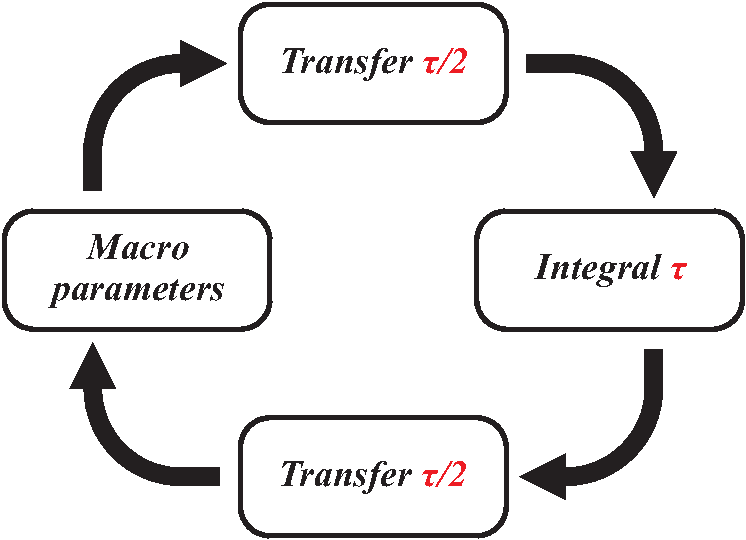
\includegraphics[width=\columnwidth]{split_scheme.pdf}
		\end{column}
	\end{columns}
\end{frame}
%	\begin{block}<2->{Макропараметры газа}

\begin{frame}
	\frametitle{Применяемые сетки}
	\begin{columns}[c]
		\column{0.5\columnwidth}
			\centering{Пространственные сетки}
			\begin{itemize}
				\item прямоугольная \\
				\smallskip
				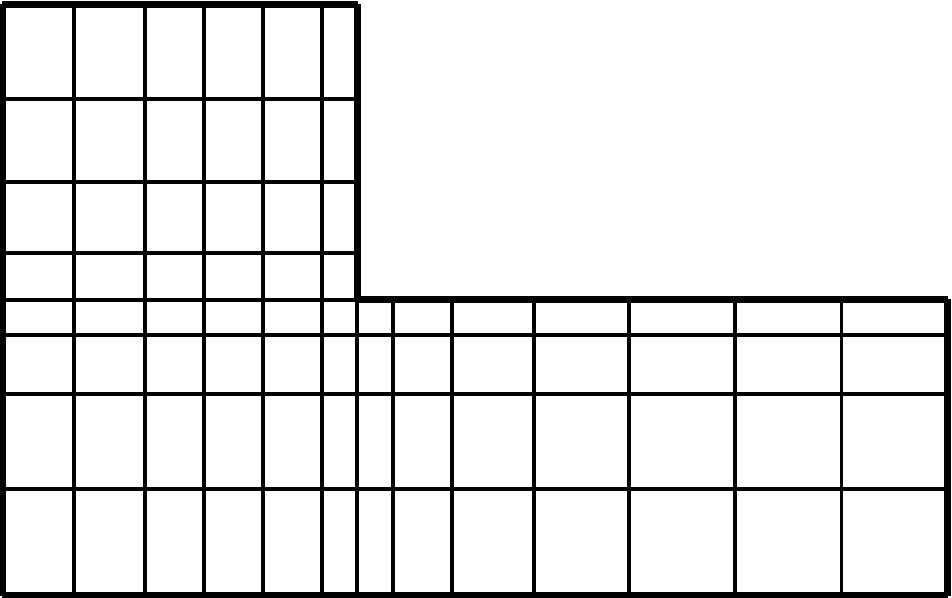
\includegraphics[width=3cm]{rectangle_mesh.pdf}
				\item тетраэдрическая \\
				\smallskip
				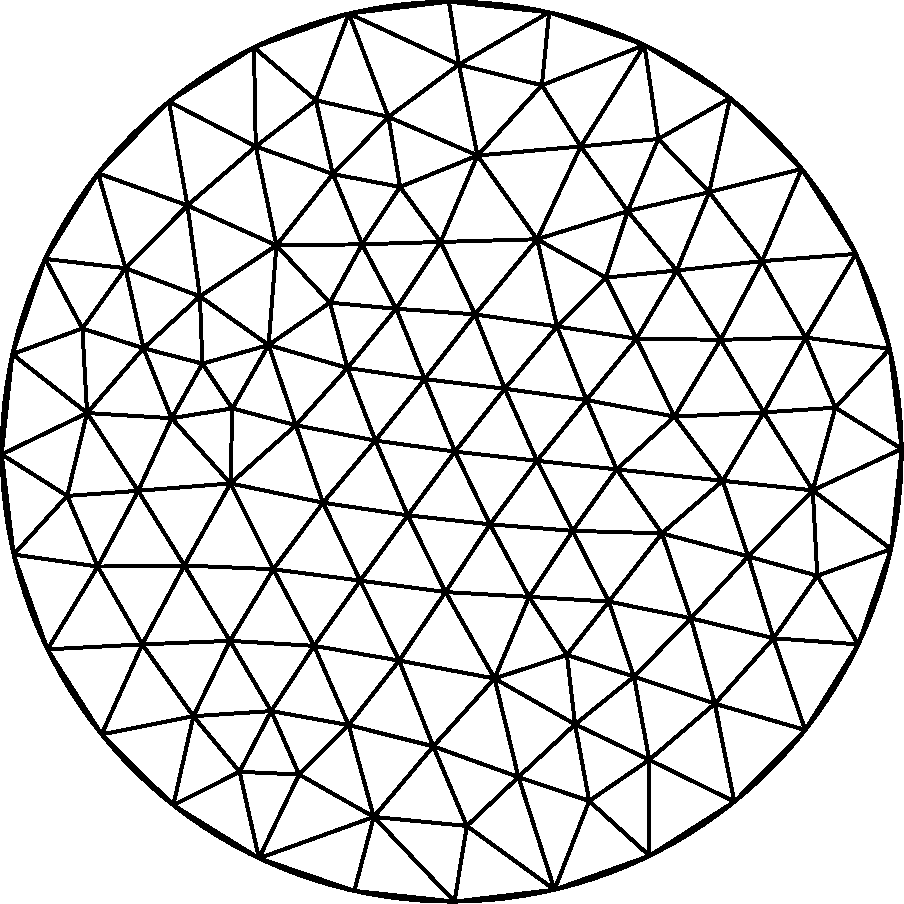
\includegraphics[width=3cm]{circle_mesh.pdf}
			\end{itemize}
		\column{0.5\columnwidth}
			\centering{Скоростная сетка\\}
			\bigskip
			\begin{tikzpicture}[scale=.25]
				\foreach \x in {-10,...,10}
					\foreach \y in {-10,...,10}
					{
						\pgfmathtruncatemacro\mynumber{\x^2+\y^2}
						\ifnum \mynumber<100
							\pgfpathrectangle{\pgfpoint{\x cm}{\y cm}}{\pgfpoint{1cm}{1cm}}
						\fi
					}
				\pgfusepath{draw}
			\end{tikzpicture}
	\end{columns}
\end{frame}

\begin{frame}
	\frametitle{Левая часть уравнения Больцмана}

	Необходимы \alert{консервативные} и \alert{монотонные} разностные схемы
	\begin{itemize}
		\item потоковая схема \alert{первого} порядка
		\[ {f^{j+1}_i-f^j_i \over \tau} = \sum\limits_i \dfrac{S_i}{V}F_i,\text{ потоки } F_i= (\boldsymbol\xi \cdot \mathbf{n}_i) f^j_p \]
		\item TVD-схема \alert{второго} порядка
		\[ {f^{j+1}_i-f^j_i \over \tau} = \xi{\tilde f_{i+1/2}-\tilde f_{i-1/2}  \over h} \]
		\[ \tilde f_{i+1/2} = f^j_i+\dfrac1{2}\left(1-\dfrac{\xi\tau}{h}\right)
			\varphi\left({f^j_i-f^j_{i-1} \over f^j_{i+1}-f^j_i} \right) (f^j_{i+1}-f^j_i), \xi>0 \]
		\[\text{MC limiter: } \varphi(\theta)=\max \left[0,\min\left(2\theta,\frac{1+\theta}{2},2\right)\right] \]
	\end{itemize}
\end{frame}

\subsection{Проекционный метод}
\begin{frame}
	\frametitle{Правая часть уравнения Больцмана}
	\begin{itemize}
		\item симметризация интегрирование по \(\boldsymbol\xi\) и \(\boldsymbol\xi'_1\)
			\[
				J(\boldsymbol\xi_\gamma) = \int\delta(\boldsymbol\xi-\boldsymbol\xi_\gamma)
				(f_1' f' - f_1 f) gb \dd{b} \dd\varepsilon \dd\boldsymbol\xi \dd\boldsymbol\xi_1
			\]
		\item переход от интегрирования к суммированию
			\[ \int\dots\dd{b}\dd\varepsilon\dd\boldsymbol\xi\dd\boldsymbol\xi_1 \to \sum\limits_{\nu=1}^{N_\nu}\dots \]
		\item 8D интегрирующая сетка Коробова \( \{b_\nu,\varepsilon_\nu,\boldsymbol\xi_{\alpha_\nu},\boldsymbol\xi_{\beta_\nu}\} \)
	\end{itemize}
	\begin{block}{}
		\textit{Черемисин Ф.Г.} Консервативный метод вычисления интеграла столкновений Больцмана
			// Доклады РАН. — 1997. — Т. 357, № 1. — С. 53—56.
%		\textit{Tcheremissine F.G.} Solution of the Boltzmann Kinetic Equation for Low Speed Flows 
%			// Transport Theory and Statistical Physics. — 2008. — V.~37, N.~5. — P. 564—575.
	\end{block}
\end{frame}

\begin{frame}
	\frametitle{Проекционный метод}
	\begin{columns}
		\begin{column}{6cm}
			\[ 
				\boldsymbol\xi_{\alpha_\nu},\boldsymbol\xi_{\beta_\nu}\in \Omega \rightarrow
				\boldsymbol\xi'_{\alpha_\nu},\boldsymbol\xi'_{\beta_\nu}\notin \Omega 
			\]
			\begin{center}
			\begin{tikzpicture}[every node/.style={circle,draw=blue!50,fill=blue!20,thick,inner sep=0pt,minimum size=8mm}, >=latex',thick, node distance=.5]
				\node (alpha) {\footnotesize\(\boldsymbol\xi_\alpha'\)};
				\node (lambda) [below left=of alpha] {\footnotesize\(\boldsymbol\xi_\lambda\)};
				\node (lambdas) [below right=of alpha] {\footnotesize\(\boldsymbol\xi_{\lambda+s}\)};
				\draw [->] (alpha) to (lambda);
				\draw [->] (alpha) to (lambdas);
			\end{tikzpicture}
			\hspace{3mm}
			\begin{tikzpicture}[every node/.style={circle,draw=blue!50,fill=blue!20,thick,inner sep=0pt,minimum size=8mm}, >=latex',thick, node distance=.5]
				\node (beta) {\footnotesize\(\boldsymbol\xi_\beta'\)};
				\node (mu) [below left=of beta] {\footnotesize\(\boldsymbol\xi_\mu\)};
				\node (mus) [below right=of beta] {\footnotesize\(\boldsymbol\xi_{\mu-s}\)};
				\draw [->] (beta) to (mu);
				\draw [->] (beta) to (mus);
			\end{tikzpicture}
			\end{center}
		\end{column}
		\begin{column}{4cm}
			\begin{tikzpicture}[scale=.4, >=latex',thick]
				\draw[step=1, gray, very thin] (-5.4,-5.4) grid (5.4,5.4);
				\draw (0,0) circle (5);
				\draw[->] (0,0)--(4,-3) node[below right] {\footnotesize\(\boldsymbol\xi_\alpha\)};
				\draw[->] (0,0)--(-4,3) node[above left] {\footnotesize\(\boldsymbol\xi_\beta\)};
				\draw[->] (0,0)--(4.77,1.5);
				\draw[->] (0,0)--(-4.77,-1.5);
				\draw (-5,-2) circle (.1) node[anchor=north] {\footnotesize\(\boldsymbol\xi_{\lambda+s}\)};
				\draw (-4,-1) circle (.1) node[anchor=south] {\footnotesize\(\boldsymbol\xi_\lambda\)};
				\draw (5,2) circle (.1) node[anchor=south] {\footnotesize\(\boldsymbol\xi_{\mu-s}\)};
				\draw (4,1) circle (.1) node[anchor=north] {\footnotesize\(\boldsymbol\xi_\mu\)};
			\end{tikzpicture}
		\end{column}
	\end{columns}
	Регуляризация функций распределения разлетных скоростей:
	\[\left\{ \begin{array}{l l}
		\delta(\xi_{\alpha_\nu}'-\xi_\gamma) = (1-{\color{blue}r_\nu}) \delta(\xi_{\lambda_\nu} - \xi_\gamma) + {\color{blue}r_\nu} \delta(\xi_{\lambda_\nu+s} - \xi_\gamma)  \\
		\delta(\xi_{\beta_\nu}'-\xi_\gamma) = (1-{\color{blue}r_\nu}) \delta(\xi_{\mu_\nu} - \xi_\gamma) + {\color{blue}r_\nu} \delta(\xi_{\mu_\nu-s} - \xi_\gamma)  \\
	\end{array}\right. \]
	\[(\xi_{\alpha_\nu}') ^ 2 + (\xi_{\beta_\nu}') ^2 = (1 - {\color{blue}r_\nu}) (\xi_{\lambda_\nu} ^ 2 + \xi_{\mu_\nu} ^2) +
	{\color{blue}r_\nu} (\xi_{\lambda_\nu+s} ^ 2 + \xi_{\mu_\nu-s} ^2)\]
	\[f_{\alpha_\nu}' f_{\beta_\nu}' = (f_{\lambda_\nu} f_{\mu_\nu})^{1 - {\color{blue}r_\nu}} + (f_{\lambda_\nu+s} f_{\mu_\nu-s})^{{\color{blue}r_\nu}}\]
\end{frame}

\section{Программная реализация}
\subsection{Модульная структура}
\begin{frame}
	\frametitle{Структура программы}
	\begin{columns}
	\column{\paperwidth}
	\begin{center}
	\begin{tikzpicture}[every node/.style={shape=rectangle split,rectangle split parts=2,rounded corners,draw=blue!50,fill=blue!20,thick,inner sep=5pt,
						minimum size=1cm,node distance=1cm,text width=3cm,text badly centered}, >=latex',thick]
		\node[shape=rectangle] (solver)				{\Large\textbf{SOLVER}};
		\node[shape=rectangle] (geometry)[left=of solver]	{\textbf{геометрия \\ \smallнач. условия}};
		\node (mesh)	[above left=of solver] 	{\textbf{сетки} \nodepart{second}\footnotesize прямоугольные неструктурные};
		\node (scheme)	[above=of solver] 	{\textbf{разностные схемы} \nodepart{second}\footnotesize первого порядка TVD-схема цилиндрическая};
		\node (integral)[above right=of solver]	{\textbf{интеграл столкновений} \nodepart{second}\footnotesize одноатомный газ многоатомный газ смеси};
		\node (parallel)[right=of solver] 	{\textbf{параллельные вычисления} \nodepart{second}\footnotesize MPI \\ CUDA};
		\node (visual)	[below=of solver] 	{\textbf{визуализация} \nodepart{second}\footnotesize Gnuplot Paraview NCL};
		\draw [->] (geometry) to (solver);
		\draw [->] (mesh) to (solver);
		\draw [->] (scheme) to (solver);
		\draw [->] (integral) to (solver);
		\draw [->] (parallel) to (solver);
		\draw [->] (solver) to (visual);
	\end{tikzpicture}
	\end{center}
	\end{columns}
\end{frame}

%%%%%%%%%%%%%%%%%%%%%% Денис %%%%%%%%%%%%%%%%%%%%%%%%%%%%%%%%%
\subsection{GMSH}
\begin{frame}
	\frametitle{Неструктурированные сетки}
	\begin{columns}
	\column{0.7\columnwidth}
		{\Large \textcolor{green}{GMSH} - генератор трехмерных неструктурированных сеток} 
		\newline Авторы: \textcolor{magenta}{Christophe Geuzaine\newline Jean-François Remacle\newline} 
	\column{0.3\columnwidth}
%		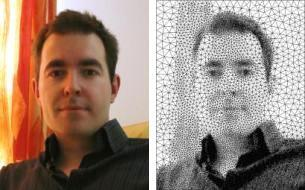
\includegraphics[width=\columnwidth]{author.png}
	\end{columns}
	\begin{itemize}
	\item открытый программный код \url{http://geuz.org/gmsh/}
	\item удобный и простой интерфейс
	\item возможность параметрического задания геометрии
	\item быстрый и надежный инструмент для построения неструктурированных сеток
	\item взаимодействие с внешними солверами 
	\end{itemize}
	\textit{C. Geuzaine and J.-F. Remacle, Gmsh: a three-dimensional finite element mesh generator with built-in pre- and post-processing facilities. International Journal for Numerical Methods in Engineering, Volume 79, Issue 11, pages 1309-1331, 2009}
\end{frame}

\subsection{}
\begin{frame}
	\frametitle{Качество неструктурированных сеток}
	\begin{columns}
	\column{0.4\columnwidth}
	Улучшение качества элеметнов сетки:
	\begin{enumerate}
	\item оптимизатор GMSH
	\item оптимизатор Netgen
	\end{enumerate}
	\column{0.75\columnwidth}
		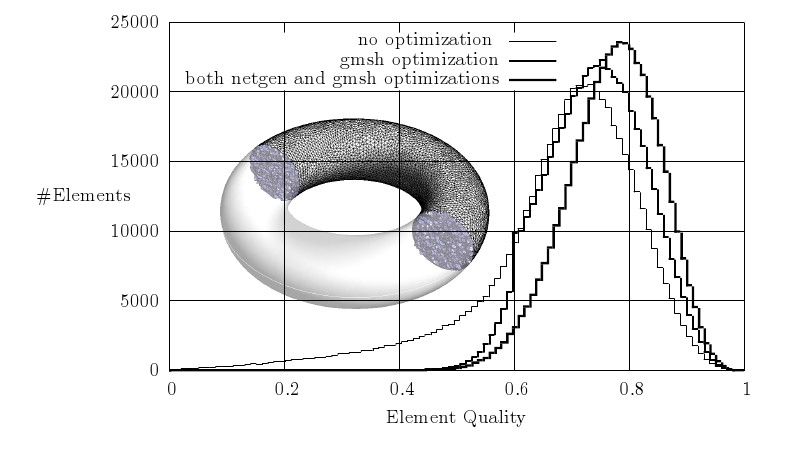
\includegraphics[width=\columnwidth]{optimizers.png}
	\end{columns}
	\textcolor{cyan}{Качество тетраэдра} $\gamma=6 \sqrt{6} (V/\displaystyle\sum_{i=1}^4 S_i L)$, $\gamma \in (0,1]$\newline
	$\gamma = 1$ для равностороннего тетраэдра,\newline
	$V$ - объем тетраэдра,\newline 
	$S_i$ - площадь $i$-й грани,\newline 
	$L$ - длина самого длинного ребра.\newline 
\end{frame}

\section{Результаты моделирования}

\subsection{}
\begin{frame}
	\frametitle{Виды молекулярных термонасосов}	
	\begin{center}
	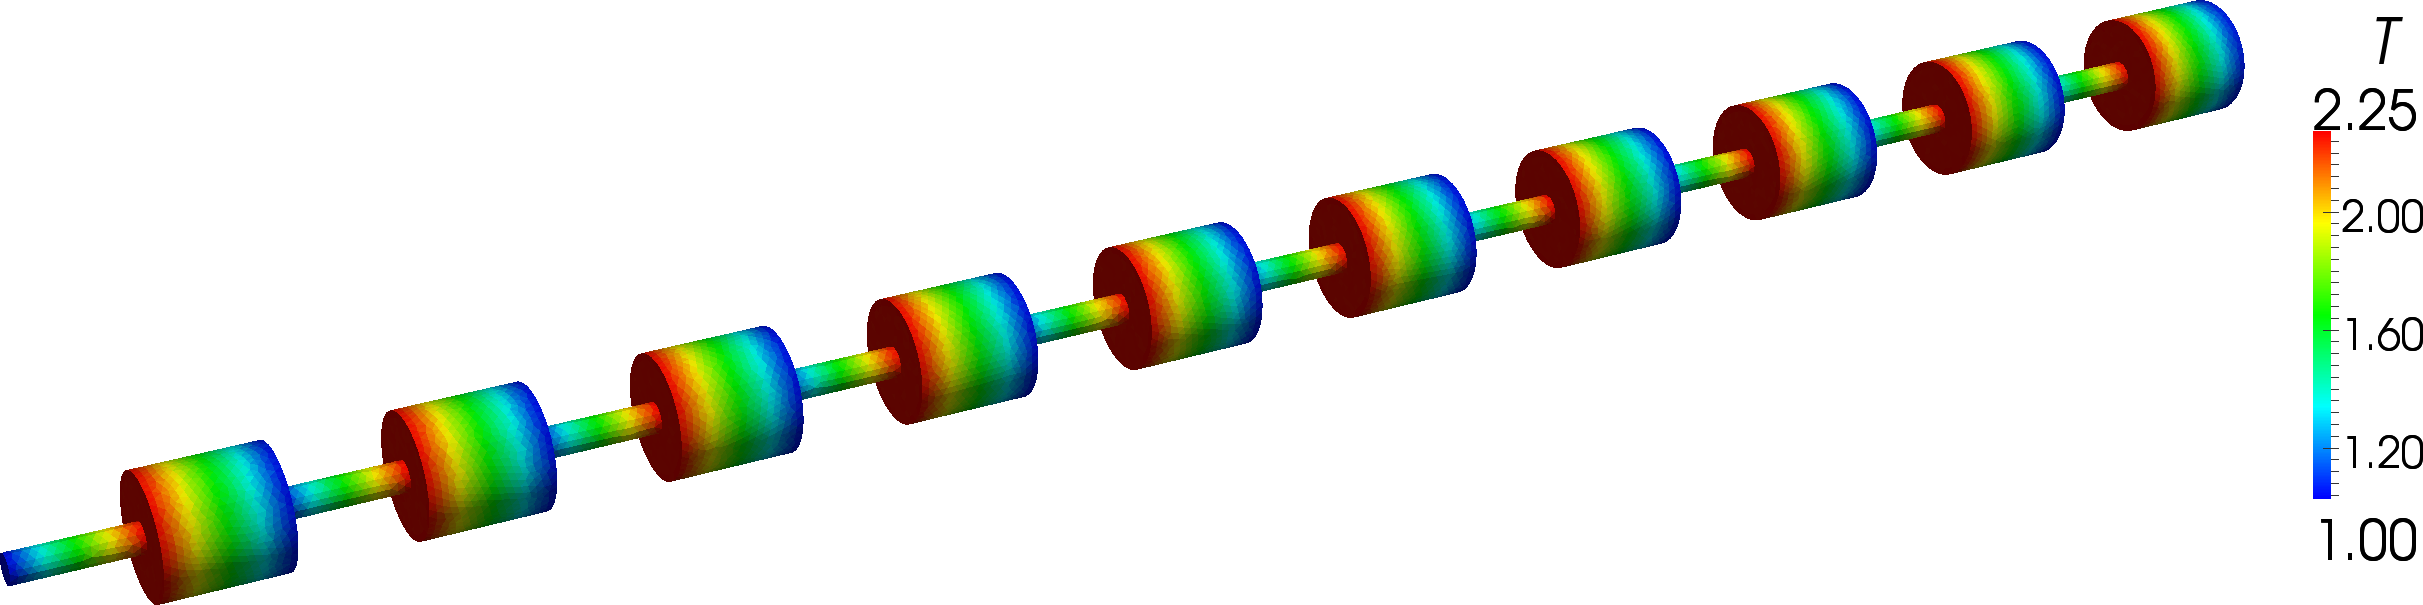
\includegraphics[width=0.7\columnwidth]{Klassic.png}
	\end{center}
	{\footnotesize \textit{Аникин Ю.А., Клосс Ю.Ю., Мартынов Д.В., Черемисин Ф.Г. Компьютерное моделирование и анализ эксперимента Кнудсена 1910 года // Нано- и микросистемная техника. — 2010 (поступила в печать)}}
	\begin{center}
	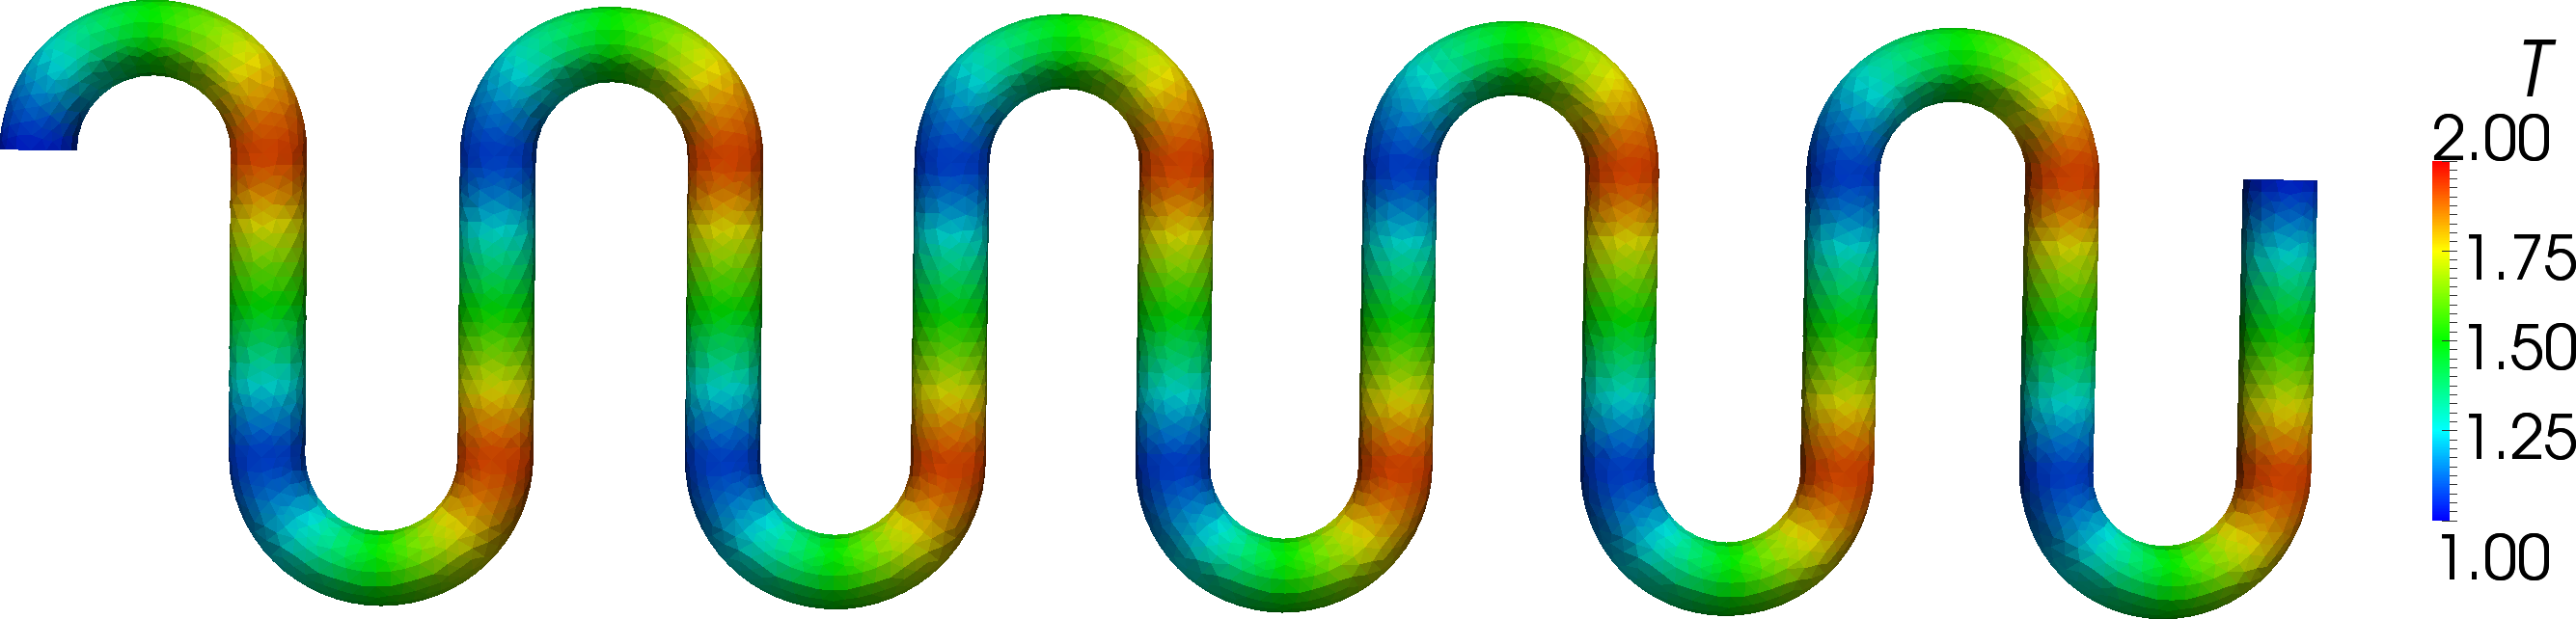
\includegraphics[width=0.7\columnwidth]{Snake.png}
	\end{center}
	{\footnotesize \textit{Клосс Ю.Ю., Мартынов Д.В., Черемисин Ф.Г. Компьютерное моделирование и анализ технических характеристик молекулярных термонасосов. // Журнал технической физики. — 2010 (поступила в редакцию)}}
\end{frame}


\begin{frame}
	\frametitle{Геометрия задачи}
	\textcolor{green}{Схема насоса} 
	\begin{columns}[c]
	\column{0.55\paperwidth}
	\begin{itemize}
	\item в начальный момент функция распределения максвелловская
	\item граничные условия
	\begin{itemize}
	\item диффузное отражение
	\item зеркальное отражение
	\end{itemize}
	\end{itemize}
	\column{0.4\paperwidth}
		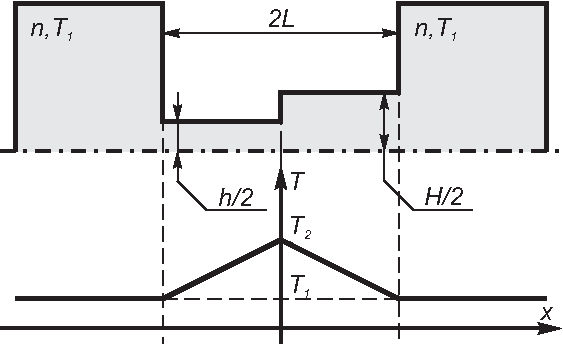
\includegraphics[width=\columnwidth]{pump_scheme.pdf}
	\end{columns}
	\textcolor{green}{Тетраэдрическая сетка} 
	\begin{columns}[c]
	\column{0.55\paperwidth}
	\begin{itemize}
		\item переменная подробность сетки
		\item алгоритм построения сетки Frontal
		\item качество сетки улучшено оптимизаторами GMSH и Netgen
	\end{itemize}
	\column{0.4\paperwidth}
		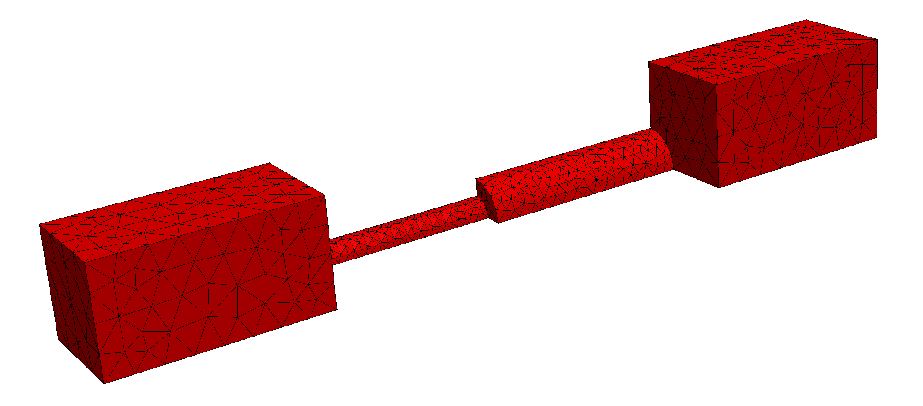
\includegraphics[width=\columnwidth]{Mesh}
	\end{columns}
\end{frame}

\subsection{Динамика процесса}
\begin{frame}
	\frametitle{Стационарные потоки}
	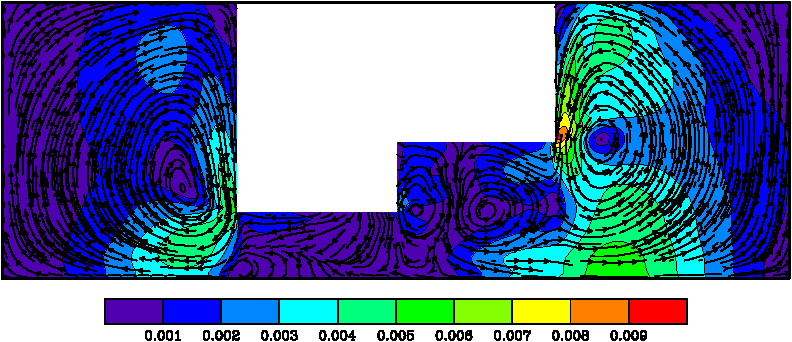
\includegraphics[width=\columnwidth]{flows.pdf}
%	\frame{
%		\movie[width=10cm, height=5cm, autostart]{}{video.avi}
%	}
\end{frame}

\begin{frame}
	\frametitle{Зависимость отношения давлений от времени}
	\begin{figure}[c]
		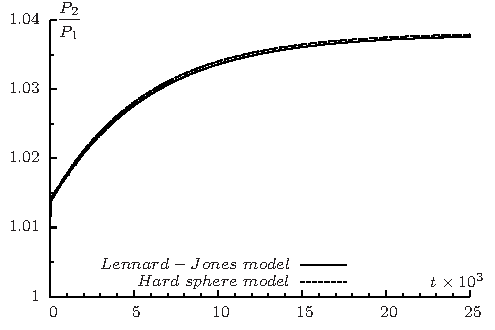
\includegraphics[width=\columnwidth]{p2t}
	\end{figure}
\end{frame}

\subsection{Стационарные распределения}
\begin{frame}
	\frametitle{Распределение макропараметров}
	\begin{columns}[c]
	\column{0.5\columnwidth}
	\begin{figure}
		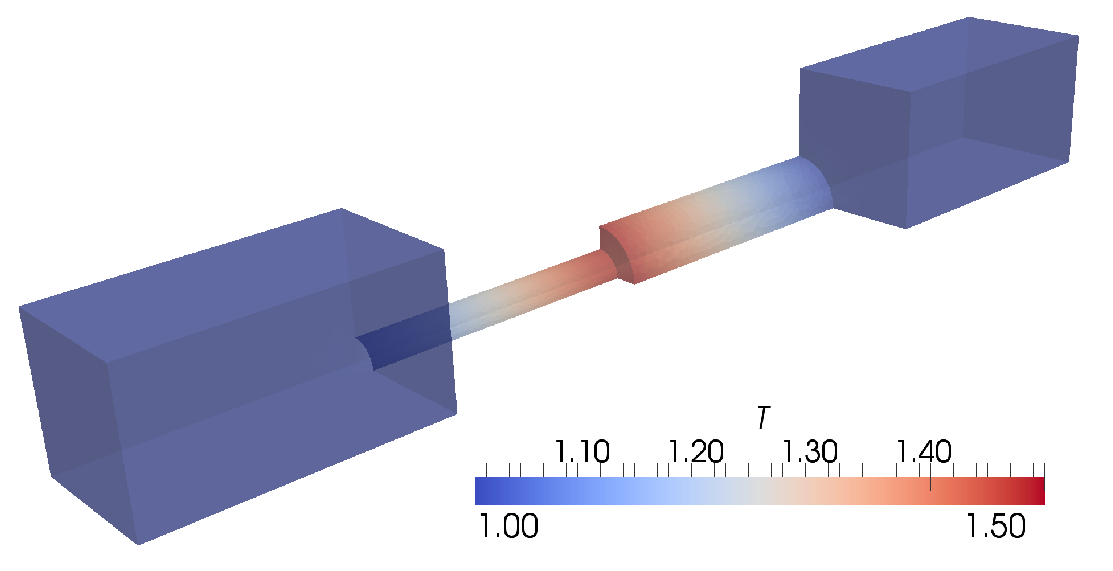
\includegraphics[height=0.25\paperheight]{T_3D}\newline
		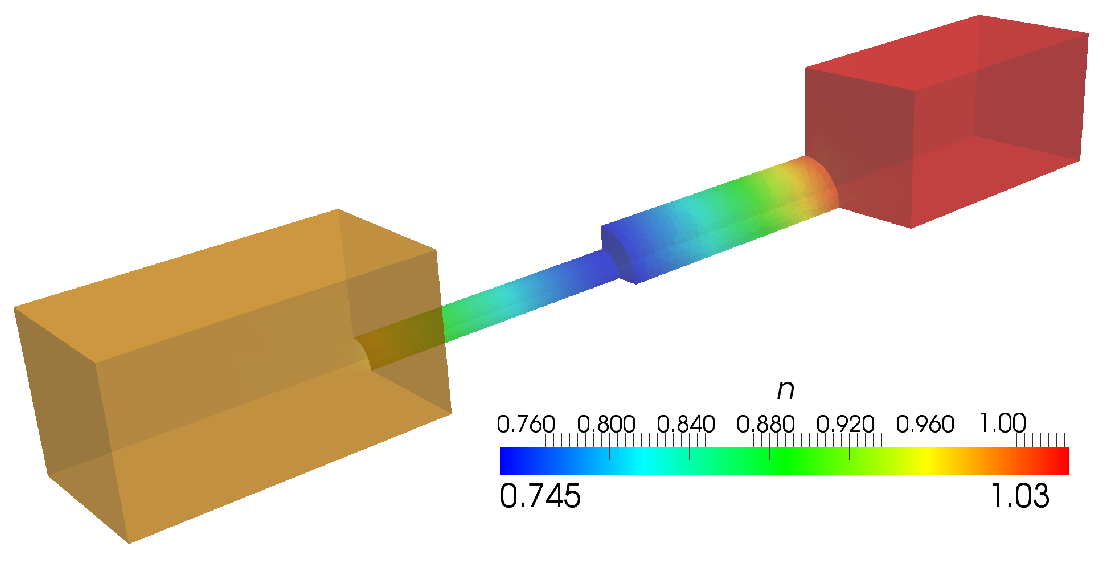
\includegraphics[height=0.25\paperheight]{n_3D}\newline
		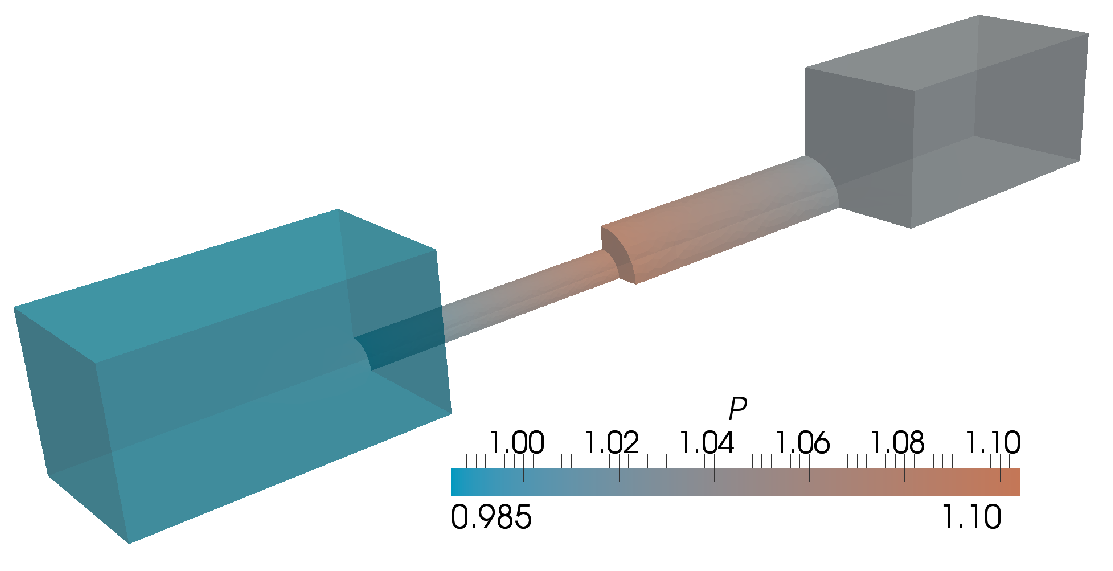
\includegraphics[height=0.25\paperheight]{P_3D}\newline
	\end{figure}
	\column{0.35\columnwidth}
		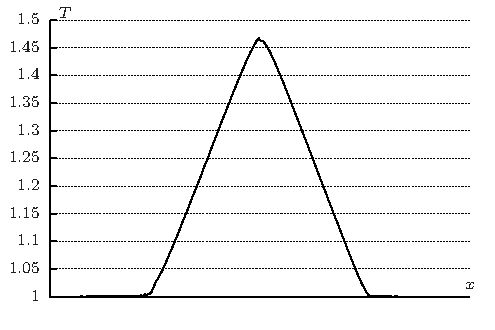
\includegraphics[height=0.25\paperheight]{1kT2x}\newline
		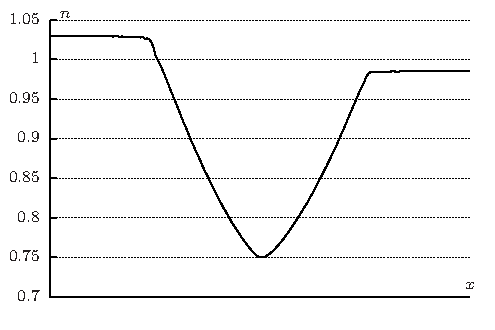
\includegraphics[height=0.25\paperheight]{1kn2x}\newline
		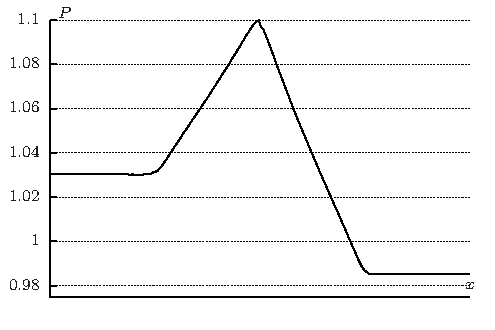
\includegraphics[height=0.25\paperheight]{1kP2x}\newline
	\end{columns}
\end{frame}

\begin{frame}
	\frametitle{Работа насоса при различных числах Кнудсена}
	\begin{columns}[c]
	\column{0.7\paperwidth}
		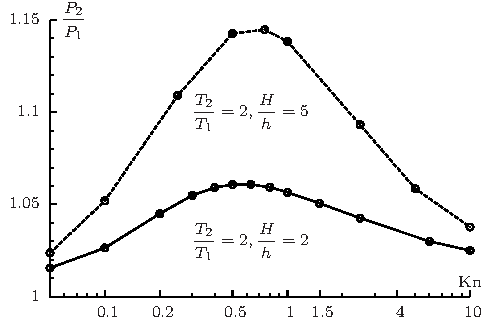
\includegraphics[width=0.7\paperwidth]{p2kn}
	\column{0.3\paperwidth}
		\begin{overpic}[width=0.28\paperwidth]{2scheme.png}
		\put(22,1){{\tiny $T_1$}}
		\put(22,14){{\tiny $T_2$}}
		\end{overpic}
	\end{columns}
\end{frame}

\begin{frame}
	\frametitle{Зависимость отношения давлений от отношения диаметров}
	\begin{columns}[c]
	\column{0.7\paperwidth}
		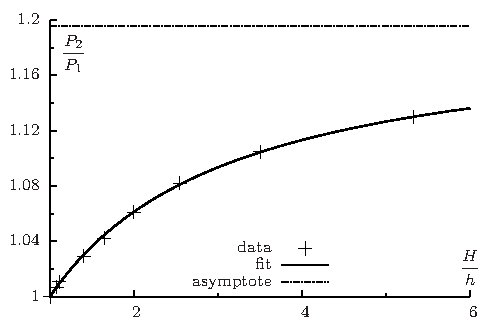
\includegraphics[width=0.7\paperwidth]{p2Hh}
	\column{0.3\paperwidth}
		\begin{overpic}[width=0.28\paperwidth]{3scheme.png}
		\put(22,1){{\tiny$T_1$}}
		\put(22,14){{\tiny$T_2$}}
		\end{overpic}
	\end{columns}
\end{frame}

\subsection{Многокаскадный насос}
\begin{frame}
	\frametitle{Многокаскадный насос}
	\begin{figure}
	\begin{overpic}[width=0.85\paperwidth]{p2x}
		\put(20,50){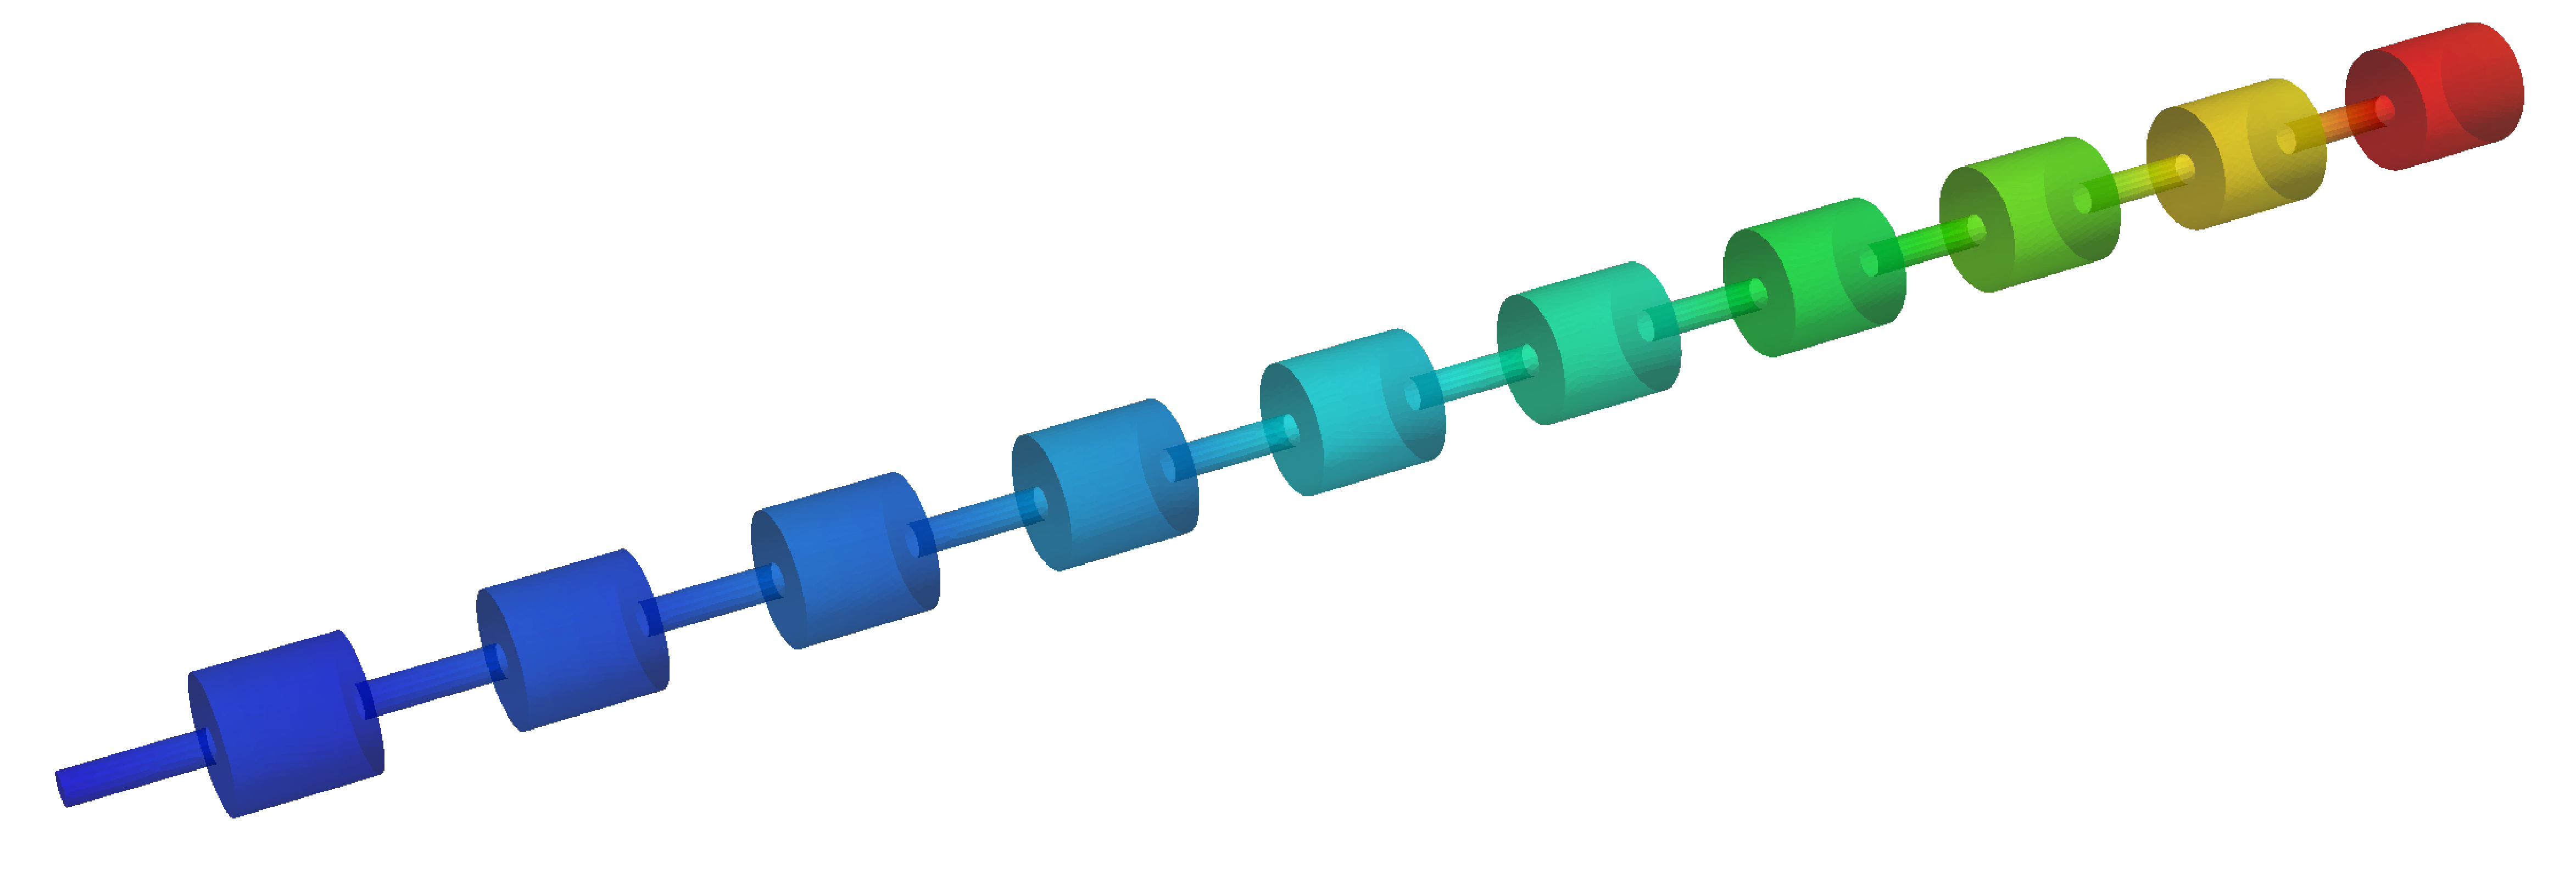
\includegraphics[width=0.55\paperwidth]{10Kaskad_P}}
	\end{overpic}
	\end{figure}
\end{frame}

\section{Заключение}
\subsection{}
\begin{frame}
	\frametitle{Проекционный метод}
	Основные преимущества проекционного метода
	\begin{itemize}
		\item дает точное решение кинетического уравнения
		\item консервативен по массе, импульсу и энергии
		\item не нарушает максвелловское распределение
		\item малый статистический шум
		\item эффективное распараллеливание
	\end{itemize}
\end{frame}

\subsection{}
\begin{frame}
	\frametitle{Программно-моделирующия среда}
	Позволяет
	\begin{itemize}
		\item решать прикладные задачи
		\item моделировать любые 2D и 3D геометрии
		\item применять различные типы пространственных сеток
		\item использовать технологии распараллелирания
		\begin{itemize}
			\item MPI
			\item GPU
		\end{itemize}
		\item красочно визуализировать результаты\newline
	\end{itemize}
	\textit{Клосс Ю.Ю., Хохлов Н.И., Черемисин Ф.Г., Шурыгин Б.А. Программно-моделирующая среда для исследования течений газа в микро- и наноструктурах на основе решения уравнения Больцмана // Атомная энергия. — 2008 — Т. 105, № 4. — С. 211–217.}
	
\end{frame}

\subsection{}
\begin{frame}
	\frametitle{Микронасосы Кнудсена}
	Основные применения
	\begin{itemize}
		\item масс спектрометр
		\item оптический спектрометр
		\item газовый анализатор\newline
	\end{itemize}
	Преимущества перед механическими насосами
	\begin{itemize}
		\item отсутствие трения
		\item применение в микроскопических масштабах
		\item высокие прочностные свойства
		\item отсутствие масел
	\end{itemize}
\end{frame}


\end{document}
